%% results_06_analysis.tex
%% Section 6: Cross-Cutting Analysis
%% All numbers come from results_converters/ run on the RQ1+RQ2 CSV files.
%% Figures: latex/figures/rq2_f*.pdf
%% ============================================================

\section{Analysis}
\label{sec:analysis}

The previous sections reported RQ1 and RQ2 in isolation: RQ1 measured
computational scaling across feature counts using approximate methods
only; RQ2 measured approximation accuracy against an exact oracle at a
fixed 12-feature dimensionality.
This section synthesises both experiments to answer three cross-cutting
questions: how consistent are libraries when they claim to compute the
same quantity; which configurations offer the best runtime--accuracy
trade-off; and what are the practical scalability limits of each library?

% ─────────────────────────────────────────────────────────────────────────────
\subsection{Cross-Library Consistency}
\label{sec:consistency}

% ``Do different libraries claiming to compute the same thing agree?''

A prerequisite for trusting any library's output is that libraries claiming
to implement the same concept---marginal Shapley values with the same
imputer---should agree with each other.
We assess consistency at two levels: (1) agreement between
\emph{exact/reference} implementations; and (2) pairwise agreement among
\emph{approximate} methods at the highest tested budget.

\paragraph{Exact reference consistency (RQ2).}

\begin{figure}[ht]
  \centering
  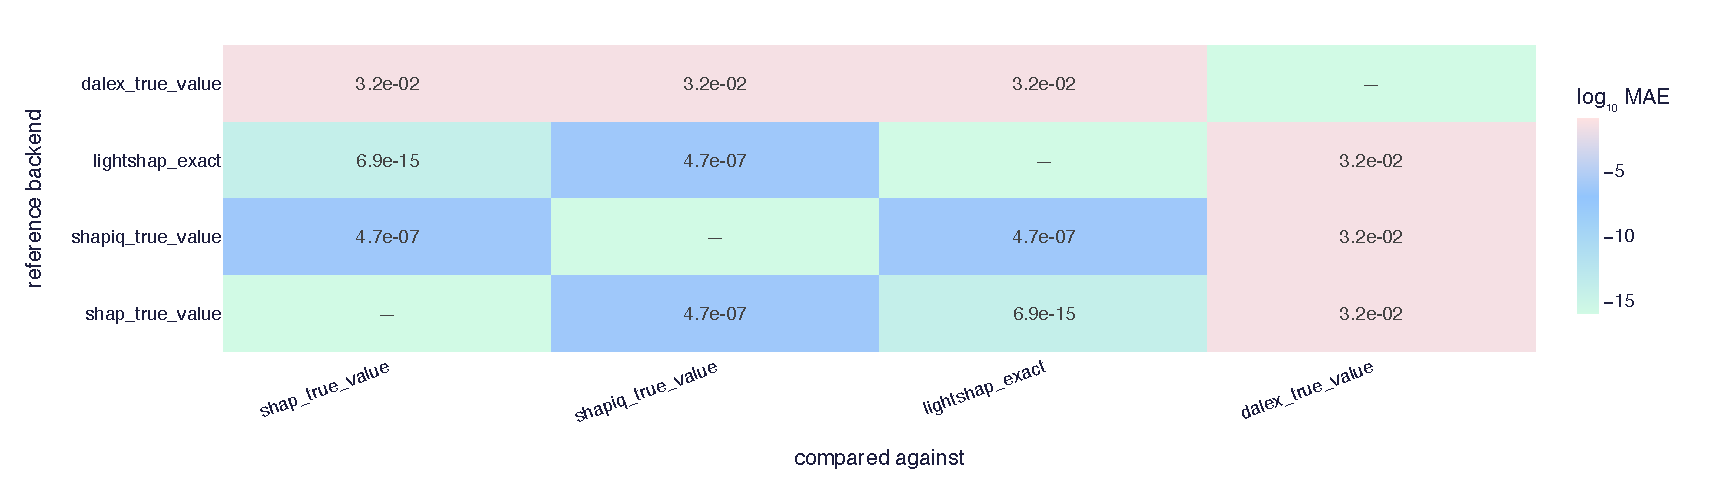
\includegraphics[width=0.72\linewidth]{figures/rq2_f5_reference_agreement}
  \caption{%
    Median relative MAE between the four exact/reference backends, aggregated
    over 200 dataset~$\times$~model~$\times$~seed cells (log\textsubscript{10}
    colour scale).
    Green cells indicate machine-precision agreement; red cells indicate
    percent-level disagreement.
    Diagonal cells are self-comparisons (undefined; shown as~``---'').
  }
  \label{fig:rq2-reference}
\end{figure}

Figure~\ref{fig:rq2-reference} and Table~\ref{tab:reference} show that
\textbf{three of the four reference implementations form a numerically
identical group}: \texttt{shap\_true\_value}, \texttt{lightshap\_exact},
and \texttt{shapiq\_true\_value} agree to a median relative MAE of
$4.7{\times}10^{-7}$ or below.
By contrast, \texttt{dalex\_true\_value} deviates from the other three by
a \textbf{median relative MAE of 3.2\,\%} (maximum 12.6\,\%).
The Spearman rank correlation between DALEX's reference and the other three
is 0.996, indicating that feature ranking is preserved but magnitudes
diverge substantially.

\begin{table}[ht]
  \centering
  \caption{%
    Cross-reference agreement: median relative MAE over 200 cells.
    Three implementations are numerically equivalent; DALEX deviates by
    3.2\,\% median (12.6\,\% maximum).
  }
  \label{tab:reference}
  \begin{tabular}{lcccc}
    \toprule
    & \texttt{shap} & \texttt{shapiq} & \texttt{lightshap} & \texttt{dalex} \\
    \midrule
    \texttt{shap}      & ---             & $4.7{\times}10^{-7}$ & $6.9{\times}10^{-15}$ & $3.2{\times}10^{-2}$ \\
    \texttt{shapiq}    & $4.7{\times}10^{-7}$  & ---        & $4.7{\times}10^{-7}$ & $3.2{\times}10^{-2}$ \\
    \texttt{lightshap} & $6.9{\times}10^{-15}$ & $4.7{\times}10^{-7}$ & --- & $3.2{\times}10^{-2}$ \\
    \texttt{dalex}     & $3.2{\times}10^{-2}$  & $3.2{\times}10^{-2}$ & $3.2{\times}10^{-2}$ & --- \\
    \bottomrule
  \end{tabular}
\end{table}

This finding has a practical implication: \emph{``exact Shapley value'' is
not a single well-defined quantity across libraries.}
DALEX applies a different background distribution or coalition-value
convention that shifts all attributions by a consistent magnitude.
All error metrics in RQ2 therefore use \texttt{shap\_true\_value} as the
oracle, and the DALEX reference is treated as a separately-calibrated
reference in the Pareto plot (Section~\ref{sec:pareto}).

\paragraph{Approximate method consistency (RQ1).}

In the dimensionality experiment, where no exact reference exists, we use
pairwise Spearman rank correlation across all 14 method configurations in
the same dataset~$\times$~model~$\times$~seed~$\times$~feature-count cell
as a consensus proxy.
At 256 features (budget 1\,024, LightSHAP capped runs excluded), the
mean cross-method consensus $\rho$ ranges from 0.34 (SHAP kernel) to 0.85
(DALEX and SHAP permutation), indicating that methods increasingly
disagree at high dimensionality.
This may reflect budget starvation: at $M=256$ a budget of 1\,024
samples fewer than 0.4\,\% of all coalitions, so different methods explore
disjoint subsets and their estimates drift apart.

\finding{%
  Three of the four exact reference implementations (SHAP, \shapiq,
  LightSHAP) agree to numerical precision; DALEX's reference deviates by
  a median 3.2\,\%.
  Among approximate methods, cross-library agreement decreases markedly
  at 256 features, suggesting budget starvation rather than implementation
  errors.%
}

% ─────────────────────────────────────────────────────────────────────────────
\subsection{Performance--Accuracy Trade-Off}
\label{sec:pareto}

\begin{figure}[ht]
  \centering
  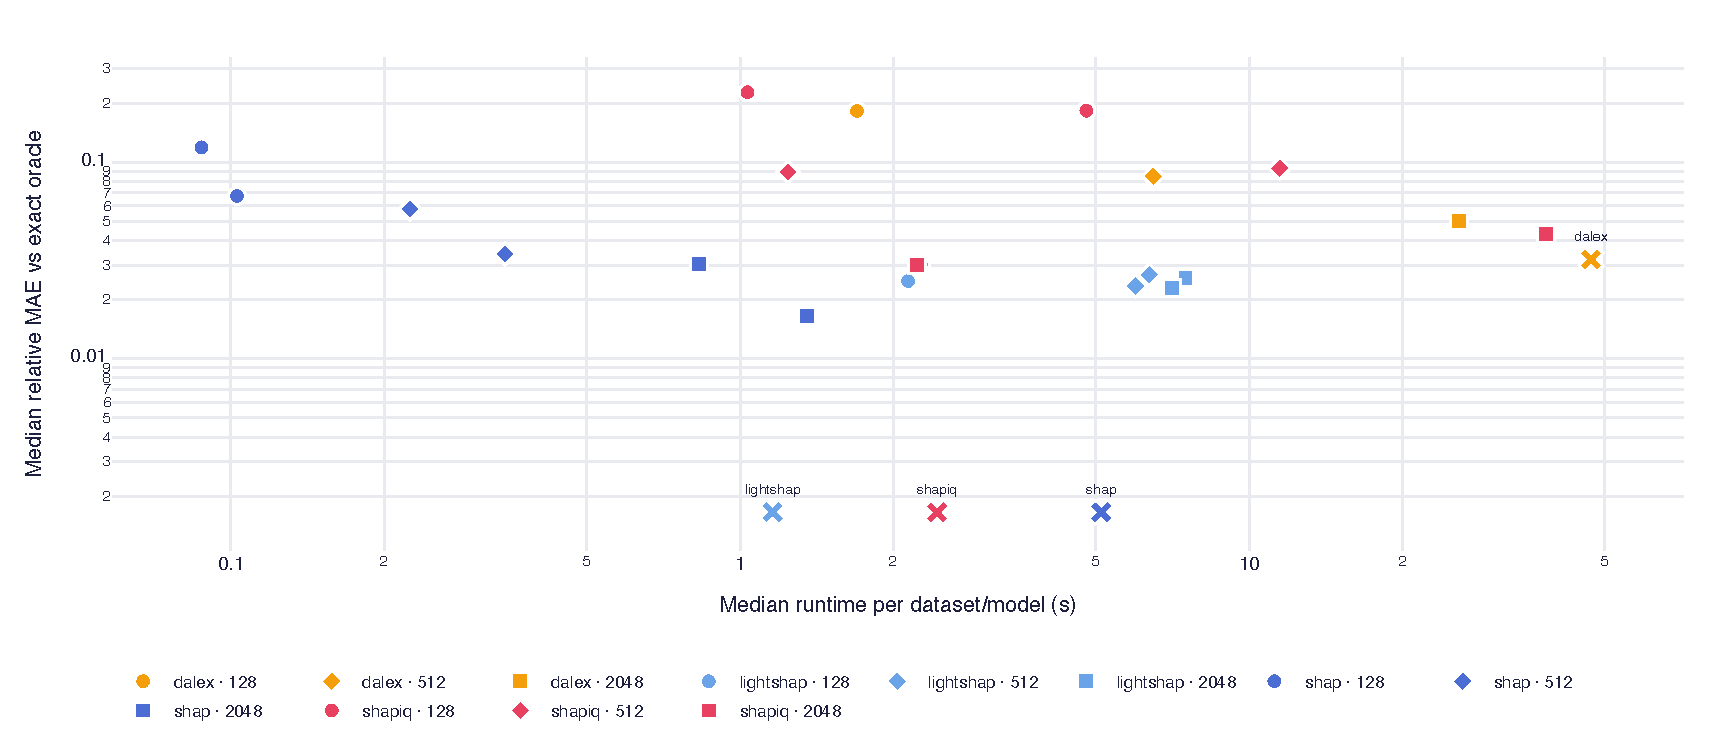
\includegraphics[width=\linewidth]{figures/rq2_f2_pareto}
  \caption{%
    Median runtime vs.\ median relative MAE for all 21 approximation
    configurations and the four exact/reference backends (cross markers,
    placed at their measured deviation from the oracle --- exact backends with
    zero true error are shown at the axis floor).
    Marker shape encodes budget: circle~=~128, diamond~=~512, square~=~2\,048.
    Medians are over five datasets~$\times$~four models.
    Points toward the lower-left dominate on both criteria.
  }
  \label{fig:rq2-pareto}
\end{figure}

\begin{figure}[ht]
  \centering
  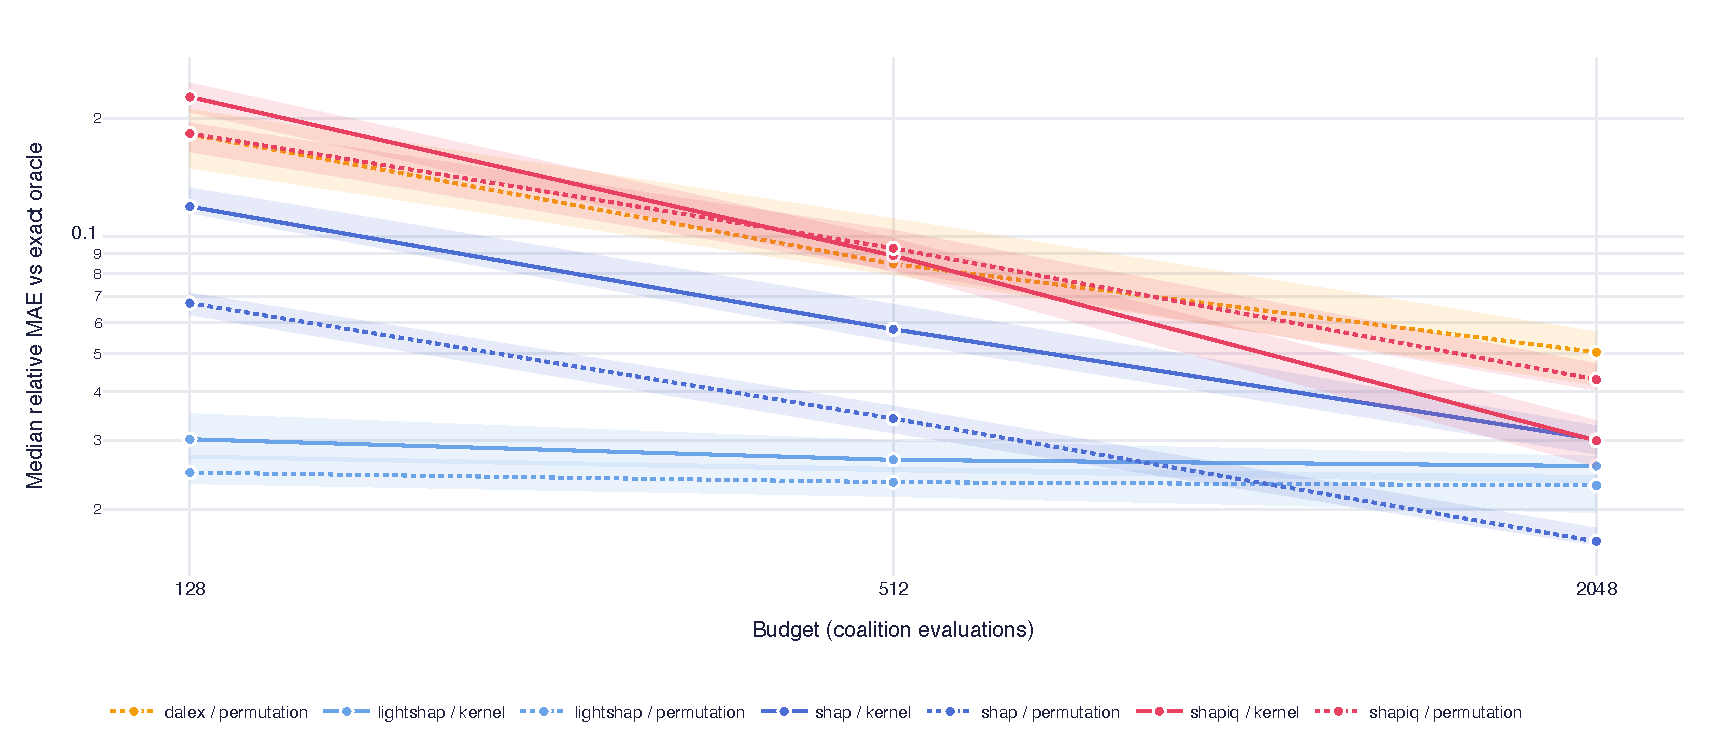
\includegraphics[width=\linewidth]{figures/rq2_f1_convergence}
  \caption{%
    Error convergence as budget increases.
    Each line is the median relative MAE vs.\ the \texttt{shap\_true\_value}
    oracle over 200 dataset~$\times$~model~$\times$~seed cells; shaded bands
    are the interquartile range across seeds.
    Dashed lines = permutation approximator; solid lines = kernel approximator.
  }
  \label{fig:rq2-convergence}
\end{figure}

Figure~\ref{fig:rq2-pareto} reveals a clear Pareto structure.
\textbf{LightSHAP} (both approximators) occupies the lower-left frontier
at every budget: at budget~128 it achieves a median relative MAE of
2.5--3.0\,\% in 2.1--2.3\,s---already close to its floor, since
increasing the budget to 2\,048 reduces error only by a factor of
$\approx 1.1{\times}$ (Figure~\ref{fig:rq2-convergence}).
\textbf{SHAP permutation} reaches the lowest error overall at budget~2\,048
(1.7\,\% in 1.4\,s), making it the best single-configuration choice when
accuracy is the priority.

The exact/reference backends show that \emph{at 12 features, computing
exact values is often cheaper than running a high-budget approximation}:
\texttt{shap\_true\_value} completes in $\approx$5.1\,s median,
\texttt{shapiq\_true\_value} in $\approx$2.4\,s, and
\texttt{lightshap\_exact} in $\approx$1.2\,s.
High-budget \shapiq\ permutation (38\,s, 4.3\,\% error) is dominated on
both axes by \texttt{lightshap\_exact}.
This ratio will invert at higher dimensionality, where exact computation
becomes exponentially expensive; the RQ1 stress test
(Section~\ref{sec:rq1-stress}) confirms this threshold is well below 1\,000
features.

\paragraph{Convergence rates.}

Table~\ref{tab:convergence} summarises error reduction from budget~128 to
budget~2\,048.
Methods starting from a high error (e.g.\ \shapiq\ kernel: 22.7\,\% at
budget~128) benefit most from a larger budget (7.6$\times$ reduction),
while LightSHAP is already near its floor at budget~128 (1.1$\times$
reduction).
The implication for practitioners: for LightSHAP, increasing the budget
beyond 128 provides negligible accuracy gains.

\begin{table}[ht]
  \centering
  \caption{%
    Median relative MAE at budget~128 and 2\,048, and the reduction factor.
    Medians over 5 datasets~$\times$~4 models~$\times$~10 seeds.%
  }
  \label{tab:convergence}
  \begin{tabular}{lrrr}
    \toprule
    Method & MAE @ 128 & MAE @ 2048 & Reduction \\
    \midrule
    LightSHAP permutation & 2.5\,\% & 2.3\,\% & $1.1\times$ \\
    LightSHAP kernel      & 3.0\,\% & 2.6\,\% & $1.2\times$ \\
    SHAP permutation      & 6.7\,\% & 1.7\,\% & $4.1\times$ \\
    SHAP kernel           & 11.9\,\% & 3.0\,\% & $3.9\times$ \\
    DALEX permutation     & 18.2\,\% & 5.0\,\% & $3.6\times$ \\
    \shapiq\ permutation  & 18.3\,\% & 4.3\,\% & $4.3\times$ \\
    \shapiq\ kernel       & 22.7\,\% & 3.0\,\% & $7.6\times$ \\
    \bottomrule
  \end{tabular}
\end{table}

\begin{figure}[ht]
  \centering
  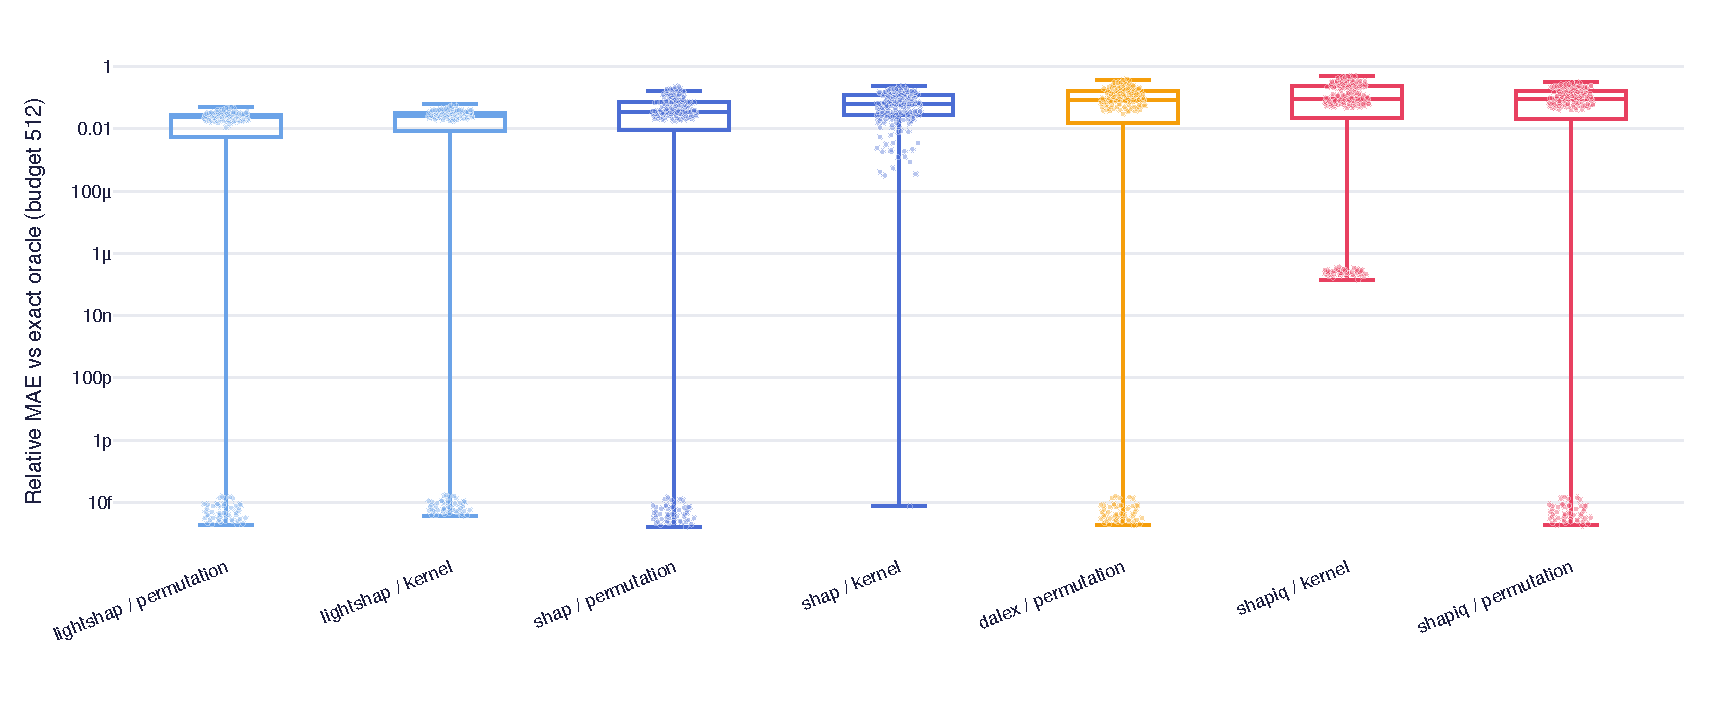
\includegraphics[width=\linewidth]{figures/rq2_f3_seed_stability}
  \caption{%
    Distribution of relative MAE across 10 seeds per method at
    budget~512 (all datasets~$\times$~models pooled; $n = 200$ points
    per method).
    Values are clamped at $10^{-15}$ (the empirical machine-precision
    floor on linear regularized cells where all methods match the oracle
    exactly).
    Tight boxes indicate reproducible estimates; long lower whiskers
    indicate machine-precision matches on structurally easy models.
  }
  \label{fig:rq2-stability}
\end{figure}

Figure~\ref{fig:rq2-stability} shows seed-level variation at budget~512.
The interquartile range divided by the median error (a normalised spread
measure) is lowest for LightSHAP kernel (0.75) and LightSHAP permutation
(0.85), confirming that these methods produce consistent estimates
regardless of the random seed.
\shapiq\ kernel has the widest relative spread (2.31), reflecting its
higher sensitivity to which coalitions happen to be sampled at a given
seed.

\finding{%
  LightSHAP provides the best accuracy-per-second at all budgets but has
  effectively converged already at budget~128 and is infeasible at
  $M \geq 79$ features.
  SHAP permutation achieves the lowest error overall at high budget (1.7\,\%)
  with short runtimes ($<$2\,s at budget~2\,048).
  At 12 features, computing exact values (lightshap\_exact: 1.2\,s,
  MAE~$\approx 0$) is cheaper than running \shapiq\ permutation
  at budget~2\,048 (38\,s, 4.3\,\% error).%
}

% ─────────────────────────────────────────────────────────────────────────────
\subsection{Scalability Summary}
\label{sec:scalability}

Table~\ref{tab:scalability} consolidates the practical limits observed
across RQ1 and RQ2.
``DNF'' (Did Not Finish) denotes configurations where at least one run
exceeded the 10-minute execution cap in the standard benchmark grid.
``Structural fail'' denotes configurations where a budget constraint
prevents the method from returning any output.
The minimum stable budget column reports the smallest budget at which
median sign agreement with the exact oracle exceeds 0.99 (from RQ2).

\begin{table}[ht]
  \centering
  \caption{%
    Practical scalability limits per library and approximator, derived from
    the RQ1 dimensionality benchmark (columns 2--3) and the RQ2 accuracy
    benchmark (columns 4--5).
    Max features = largest feature count tested without DNF or structural
    failure; ``$>$256'' means no failures in the standard grid (256 maximum).
    Min stable budget = smallest budget with median sign agreement
    $\rho_\text{sign} \geq 0.99$ vs.\ the exact oracle.%
  }
  \label{tab:scalability}
  \begin{tabular}{llcc}
    \toprule
    Library & Approx. & Max features & Min stable budget \\
    \midrule
    SHAP & kernel      & $>$256           & 2\,048 \\
    SHAP & permutation & 256 (512 fail)$^a$ & 2\,048 \\
    \shapiq & kernel   & $>$256           & $>$2\,048 \\
    \shapiq & permutation & $>$256        & $>$2\,048 \\
    LightSHAP & kernel & $\approx$64$^b$  & $>$2\,048 \\
    LightSHAP & permutation & $\approx$64$^b$ & 128 \\
    DALEX & permutation & $>$256          & 2\,048 \\
    \bottomrule
    \multicolumn{4}{l}{\footnotesize $^a$ Budget~512 fails at $M \geq 257$ ($2M+2 > 512$); budget~1\,024 succeeds.} \\
    \multicolumn{4}{l}{\footnotesize $^b$ DNF in 12.5\,\% of runs at 79 features; 63--75\,\% at 256 features.} \\
  \end{tabular}
\end{table}

% ─────────────────────────────────────────────────────────────────────────────
\subsection{API and Reproducibility Notes}
\label{sec:api}

The following issues were discovered during benchmarking and are
relevant for practitioners intending to reproduce or extend these results.

\paragraph{Parameter naming inconsistency.}
Budget is specified via different keyword arguments across libraries:
\texttt{nsamples} (SHAP), \texttt{budget} (\shapiq), \texttt{n\_samples}
(LightSHAP), and the number of iterations (DALEX).
A common wrapper layer was required to ensure that all libraries received
the same effective number of model evaluations.

\paragraph{Background dataset handling.}
All four libraries were configured with $n_\text{bg} = 100$ background
samples drawn from the training set.
LightSHAP's internal background handling differs from the marginal imputer
used by SHAP and \shapiq; this contributes to the $\approx$1\,\% gap
between LightSHAP and the numerically-equivalent shap/shapiq reference
values in the accuracy experiment.

\paragraph{Structural budget constraint (SHAP permutation).}
SHAP's \texttt{Permutation\-Explainer} requires a budget of at least
$2M + 2$ evaluations to complete one full permutation pass.
At $M = 256$ features this is 514 evaluations, which exceeds budget~512
and causes the explainer to return without computing.
This is not a crash or timeout: the function returns silently with no
output.
Practitioners using budget-constrained SHAP permutation should verify that
budget~$> 2M + 2$ before relying on the results.

\paragraph{Numerical precision differences.}
DALEX's \texttt{true\_value} backend disagrees with the other three exact
implementations by a median 3.2\,\% relative MAE and up to 12.6\,\%
in the worst cell.
This difference is systematic across all 200 dataset~$\times$~model
cells and is attributable to DALEX's default coalitional value function
rather than floating-point rounding.
Users comparing DALEX exact values with SHAP or \shapiq\ exact values
should not assume interchangeability.

\paragraph{LightSHAP execution cap.}
LightSHAP's kernel approximator appears to be the most computationally
intensive implementation tested, reaching up to 3.5\,h at 1\,000 features.
The observed runtimes cluster tightly at exactly 600\,s in the standard
benchmark grid (120 of 120 time-capped runs are LightSHAP), suggesting
that a retry or timeout mechanism internal to the library saturates at
the 10-minute wall-clock limit and then continues.
